% Convex
\chapter{凸函数}
\label{chap:convex-functions}

\begin{definition}[凸函数]

  \begin{enumerate}
  \item 函数$f(x)$被称为域$\mathcal{D}$上的凸函数,若$\forall x1,x2\in\mathcal{D}, t\in[0,1]$,下面不等式成立:
    \begin{align}\label{eq:convex-defintion}
      f\left(tx_1+(1-t)x_2\right)\le tf(x_1) + (1-t)f(x_2)
    \end{align}
  \item 函数$f(x)$被称为域$\mathcal{D}$上的严格凸函数,若$\forall x1,x2\in\mathcal{D}, t\in(0,1),x_\ne x_2$,下面不等式成立:
    \begin{align}
      f\left(tx_1+(1-t)x_2\right)< tf(x_1) + (1-t)f(x_2)
    \end{align}
  \end{enumerate}
\end{definition}

从图形上看,凸函数对应的曲线上任意两点的连线在曲线之上。令$t\equiv 1-\lambda$代入,不等式\ref{eq:convex-defintion}还可以等价的写成以下形式
\begin{align*}
  f\left(x_1+\lambda(x_2-x_1)\right)\le f(x_1) + \lambda \left(f(x_2)-f(x_1)\right)
\end{align*}


\begin{figure}[htb]
  \centering
  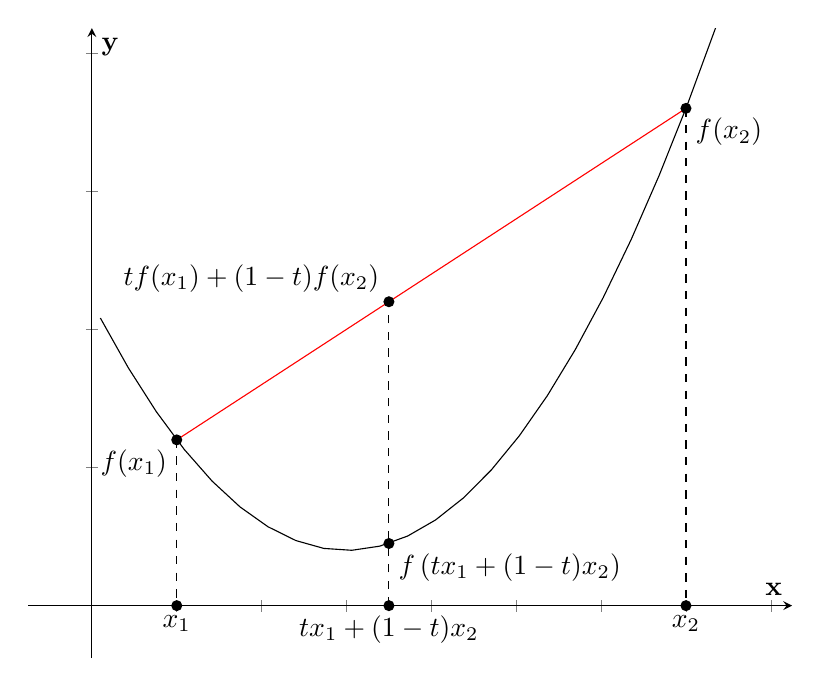
\begin{tikzpicture}[scale=1]
    \begin{axis}[
      scale only axis,
      width=0.8\textwidth,
      height=8cm,
      xmin = 0,
      xmax = 75,
      ymin = 0,
      ymax = 38, 
      axis lines = middle,
      enlargelimits = true,
      xlabel = {$\mathbf{x}$},
      ylabel = {$\mathbf{y}$},
      yticklabels={,,},
      xticklabels={,,}
      ]
      % \addplot+[mark = none] coordinates {%
      %   (0 ,40) 
      %   (20, 30)
      %   (30, 20)
      %   (35, 10)
      %   (39, 0)};
      \coordinate (A) at (axis cs:10,12);
      \coordinate (B) at (axis cs:70,36);
      \coordinate (C) at (axis cs:35,4.5);
      \coordinate (D) at (axis cs:35,22);
      \coordinate (E) at (axis cs:35,0);
      \coordinate (F) at (axis cs:10,0);
      \coordinate (G) at (axis cs:70,0);
      \addplot[domain=1:80] (\x, {0.02 * (\x * \x - 60 * \x + 900) + 4});
      \addplot[dashed](35,0)--(D);
      % \addplot[dashed](A)--(F);
      % \addplot[dashed](B)--(G);
    \end{axis}
    \draw[color=red](A)--(B);
    \fill(A) circle(2pt) node[below left] {$f(x_1)$};
    \fill(B) circle(2pt) node[below right] {$f(x_2)$};
    \fill(C) circle(2pt) node[below right] {$f\left(tx_1 + (1-t)x_2\right)$};
    \fill(D) circle(2pt) node[above left] {$tf(x_1) + (1-t)f(x_2)$};
    \fill(E) circle(2pt) node[below] {$tx_1 + (1-t)x_2$};
    \fill(F) circle(2pt) node[below] {$x_1$};
    \fill(G) circle(2pt) node[below] {$x_2$};
    \draw[dashed](A)--(F);
    \draw[dashed](B)--(G);
  \end{tikzpicture}
  \caption{凸函数}
  \label{fig:convex-function}
\end{figure}

\begin{theorem}
  若$f(x)$在$\mathcal{D}$上二次可导,那么以下条件相互等价:
  \begin{enumerate}
  \item \label{item:convex-1} $f(x)$是凸函数。
  \item \label{item:convex-2} $\forall x,y\in\mathcal{D}, f(y)\ge f(x)+f'(x)(y-x).$
  \item \label{item:convex-3} $\forall x\in\mathcal{D}, f''(x)\ge 0.$
  \end{enumerate}
\end{theorem}
\begin{proof}
  \begin{enumerate}
  \item \ref{item:convex-1}$\implies$\ref{item:convex-2}. 由于$f(x)$是凸函数,从而$\forall\lambda\in(0,1)$,有
    \begin{align*}
      &f\left(x+\lambda(y-x)\right)\le f(x)+\lambda\left(f(y)-f(x)\right)\\
      \implies & f(y)-f(x)\ge \frac{f\left(x+\lambda(y-x)\right) -  f(x)}{\lambda}\\
      \implies & f(y)-f(x)\ge \frac{f\left(x+\lambda(y-x)\right) -  f(x)}{\lambda(y-x)}\cdot(y-x)
    \end{align*}
    上式中令$\lambda\downarrow 0$,即$\Delta x\equiv\lambda(y-x)\downarrow 0$,从而有
    \begin{align*}
      f(y)-f(x)\ge \lim_{\Delta\downarrow 0}\frac{f(x+\Delta x) -  f(x)}{\Delta x}\cdot(y-x) = f'(x)(y-x)
    \end{align*}
  \item \ref{item:convex-2}$\implies$\ref{item:convex-3}.\think 请利用二阶导数定义自行证明。
  \item \ref{item:convex-3}$\implies$\ref{item:convex-1}.\think 利用中值定理自行证明。
  \end{enumerate}
  \note
  其中第\ref{item:convex-2}点说明$f$的曲线在定义域上任意一点的切线之上,
  如图~\ref{fig:convex-function-above-tangent-line}所示;
  第\ref{item:convex-3}点说明曲线的二阶导数非负,也就时说其一阶导数是单
  调增函数。
\end{proof}

\begin{figure}[htb]
  \centering
  \begin{tikzpicture}[scale=1]
    \begin{axis}[
      scale only axis,
      width=0.8\textwidth,
      height=3cm,
      xmin = 0,
      xmax = 75,
      ymin = 0,
      ymax = 27, 
      axis lines = middle,
      enlargelimits = true,
      xlabel = {$\mathbf{x}$},
      ylabel = {$\mathbf{y}$},
      yticklabels={,,},
      xticklabels={,,}
      ]
      \coordinate (A) at (axis cs:40,6);
      \addplot[domain=1:80] (\x, {0.02 * (\x * \x - 60 * \x + 900) + 4});
      \addplot[domain=10:60,color=red] (\x, {6 + 0.4 * (\x - 40)});
    \end{axis}
    \fill(A) circle(2pt) node[below left] {};
  \end{tikzpicture}
  \caption{凸函数示意:曲线位于任一点的切线之上}
  \label{fig:convex-function-above-tangent-line}
\end{figure}


% Jensen
\begin{theorem}
  如果$f(x)$是凸函数,那么对于$p_i\ge0$且$\sum_{i=1}^{n}p_i=1$,有
  \begin{align}
    f(\sum_{i=1}^{n}p_ix_i)\le \sum_{i=1}^{n}p_i f(x_i)
  \end{align}
\end{theorem}

\begin{proof}
  事实上,Jensen不等式与凸函数的定义是等价的,即若函数$f(x)$是凸函数,
  当且仅当$f(x)$满足Jensen不等式。
  \begin{enumerate}
  \item 充分性。在Jensen不等式中令$n=2$,可知$f(x)$满足凸函数定义,从而是凸函数。
  \item 必要性。设$f(x)$是凸函数,$n=2$时Jensen不等式即是凸函数定义中的条件,即Jensen不等式在$n=2$时成立。
    设Jensen不等式对$n\le K$时成立,考虑$n=K+1$的情况。关键点,把其中两项凑成一项,从而$K+1$项变成$K$项,可利用$n\le K$时成立的结论。令
    \begin{align*}
      p_K'&\equiv p_K+p_{K+1}\\
      x_K'&\equiv\frac{p_K}{p_K'}x_K + \frac{p_{K+1}}{p_K'}x_{K+1}\in[\min{(x_K, x_{K+1})}, \max{(x_K, x_{K+1})}]
    \end{align*}
    则有$p_K'x_K' = p_Kx_K + p_{K+1}x_{K+1}$,且
    \begin{align*}
      f\left(\sum_{i=1}^{K+1}p_ix_i\right) &= f\left(\sum_{i=1}^{K-1}p_ix_i  + p_K'x_K'\right)\\
      &\le \left(\sum_{i=1}^{K-1}p_if(x_i)\right) + p_K' f(x_K')\\
      &\le \left(\sum_{i=1}^{K-1}p_if(x_i)\right) + p_K'\left( \frac{p_K}{p_K'}f(x_K) + \frac{p_{K+1}}{p_K'}f(x_{K+1}) \right) \\
      &= \left(\sum_{i=1}^{K+1}p_i f(x_i)\right)
    \end{align*}
    此处没有考虑$p_K'=0$的情况,请自行补充完整。
  \end{enumerate}
  
  \note $p_K'$和$x_K'$是如何凑出来的?令$p_K'x_K' = p_Kx_K + p_{K+1}x_{K+1}$,
  且$p_K'$需满足$\sum_{i=1}^{K-1}p_i + p_K'=1$,从而可得。
\end{proof}

{\color{red}下面这个是对的吗?}
\begin{theorem}
  $f(x)$是$\mathcal{D}$上的严格凸函数,当且仅当对$\forall n\in\mathcal{Z}^+, x_i\in\mathcal{D}, p_i>0, \sum_{i=1}^{n}p_i=1$,以下不等式成立:
  \begin{align*}
    f\left(\sum_{i=1}^{n} p_i x_i\right) < \sum_{i=1}^{n} p_i f(x_i)
  \end{align*}
\end{theorem}


\begin{lemma}\label{lemma:convexity-extension}
  若$f(x)$是$[a,b]$上的连续函数,且在$(a,b]$上是凸的,则$f(x)$在$[a,b]$上是凸函数。
\end{lemma}
\begin{proof}
  下面按定义证明,即$\forall x_1,x_2\in[a,b], 0\le t\le1$,需要证明
  \begin{align*}
    f\left(tx_1 + (1-t)x_2\right) \le tf(x_1) + (1-t)f(x_2)
  \end{align*}
  若$x_1$和$x_2$都不等于$a$,那么由条件$f(x)$在$(a,b]$上严格凸可知上面不等式成立。下面不妨设$a=x_1<x_2\le b$。由连续性,可取到序列$c_i$,使得$\forall i, a=x_1<c_i\le b$,且$\lim c_i = x_1$,从而对于$c_i$和$x_2$,有
  \begin{align*}
    f\left(tc_i + (1-t)x_2\right) \le tf(c_i) + (1-t)f(x_2)
  \end{align*}
  上式中两边对$i$取极限,并由$f(x)$的连续性,有
  \begin{align*}
    \lim_{i\to\infty}f\left(tc_i + (1-t)x_2\right) &\le \lim_{i\to\infty} tf(c_i) + (1-t)f(x_2)\\
    f\left(\lim_{i\to\infty}\left(tc_i + (1-t)x_2\right)\right) &\le tf( \lim_{i\to\infty} c_i) + (1-t)f(x_2)\\
    f\left(tx_1 + (1-t)x_2\right) &\le tf(x_1) + (1-t)f(x_2)
  \end{align*}
\end{proof}

\think 上面引理对严格凸函数是否还能保持严格凸性?

\begin{lemma}\label{lemma:convexity-of-power-function}
  对$p>1$,函数$f(x)\equiv\left|x\right|^p$在$x\in\mathcal{R}$上是严格凸函数。
\end{lemma}
\begin{proof}
  函数$f(x)\equiv|x|^p$的凹凸性在图形上看是非常明显的。

  使用导数的概念证明也是非常明显的,分段考虑,$\forall x>0, f'(x) = p\left|x\right|^{p-1}>0, f''(x)=p(p-1)\left|x\right|^{(p-1)(p-2)}>0$,从而$f(x)$的一阶导数是严格单调递增的,从而$f(x)$在$(0,+\infty)$上是凸函数。同样$f(x)$在$(-\infty,0)$上也是凸函数。

  下面是初等数学的证明。

  $\forall x_1\le x_2, t\in(0,1)$,有
  \begin{align*}
    f\left(tx_1 + (1-t)x_2\right) = \left|tx_1 + (1-t)x_2\right|^p
  \end{align*}
  {\color{red}然后呢??}
\end{proof}

下面是Jensen不等式的另一种形式。
\begin{theorem}[Jensen不等式]
  若$f$是$\mathcal{D}$上的凸函数,且$\forall x_1,x_2,\cdots,x_n\in\mathcal{D}$,则
  \begin{align}
    f\left(\frac{x_1+x_2+\cdots+x_n}{n}\right)\le\frac{f(x_1)+f(x_2)+\cdots+f(x_n)}{n}
  \end{align}
  若$f$还是严格凸的,则当且仅当$x_1=x_2=\cdots=x_n$时等号成立。
\end{theorem}

\begin{proof}
  {\color{red}请证明两种形式的Jensen不等式是等价的。}
\end{proof}

\begin{example}
  对$\triangle ABC$,证明:
  \begin{align*}
    \sin A + \sin B + \sin C \le \frac{3\sqrt3}{2}
  \end{align*}
  且说明等号在何时成立。
\end{example}

\begin{proof}
  $f(x)\equiv\sin(x)$在$[0,\pi]$上是严格凹函数,由Jensen不等式有
  \begin{align*}
    \sin A + \sin B + \sin C \le 3\sin\frac{A+B+C}{3} = \frac{3\sqrt3}{2}
  \end{align*}
  当且仅当$A=B=C$时,即$A=B=C=\frac\pi3$时等号成立。
\end{proof}

\begin{example}
  若$a,b,c$是和为1的正数,求下式的最小值
  \begin{align*}
    \left(a+\frac1a\right)^{10} + 
    \left(b+\frac1b\right)^{10} + 
    \left(c+\frac1c\right)^{10}
  \end{align*}
\end{example}

\begin{proof}
  首先证明以下函数在$(0,1)$上是严格凸函数({\color{red}请用二次导数自行证明})
  \begin{align*}
    f(x)\equiv\left(x+\frac1x\right)^{10}
  \end{align*}
  其次利用Jensen不等式,有
  \begin{align*}
    &\left(a+\frac1a\right)^{10} + 
    \left(b+\frac1b\right)^{10} + 
    \left(c+\frac1c\right)^{10}\\
    =&   f(a) + f(b) + f(c)\\
    \ge& 3f\left(\frac{a+b+c}3\right)\\
    =&   3f{\frac13}\\
    =&   3 \left(\frac{10}{3}\right)^{10} = \frac{10^{10}}{3^9}
  \end{align*}
  当且仅当$a=b=c=\frac13$时等号成立。
\end{proof}